\begin{Example}[reagan]{Race and politics in the 1980 US Presidential vote}
\tabref{tab:reagtab} shows data (\citet[Table 4.12]{Agresti:90}, from \citet{CloggShockey:88})
from the 1982 General Social Survey on
votes in the 1980 US Presidential election for Reagan or for Carter
or other in relation to race and conservatism (1=most liberal,
7=most conservative).
The \Dset\ \pname{vote}, containing the
variables \pname{race}, \pname{cons}, \pname{votefor}, and
\pname{count} is listed in \datref{dat:vote}.

\begin{table}[htb]
 \caption{1982 General Social Survey: Reagan vs. Carter, by Race and Conservatism}\label{tab:reagtab}
 \begin{center}
 \begin{tabular}{c rr rr}
  \hline
       & \multicolumn{4}{c}{Race} \\
  Political & \multicolumn{2}{c}{White} & \multicolumn{2}{c}{Non White} \\ 
  \cline{2-5}
  Conservatism & Reagan & Carter/other  & Reagan & Carter/other \\ 
  \hline
  1 & 1 & 12 & 0 & 6 \\ 
  2 & 13 & 57 & 0 & 16 \\ 
  3 & 44 & 71 & 2 & 23 \\ 
  4 & 155 & 146 & 1 & 31 \\ 
  5 & 92 & 61 & 0 & 8 \\ 
  6 & 100 & 41 & 2 & 7 \\ 
  7 & 18 & 8 & 0 & 4 \\ 
  \hline
 \end{tabular}
 \end{center}
\end{table}


It is natural to treat vote for Reagan vs. (Carter or other) as the response,
and race and conservatism as predictors in this $2 \times 2 \times 7$
table, with variables VoteFor ($V$), Race ($R$) and Conservatism ($C$).
Before fitting models, it is useful to take an exploratory look
at the data.
The fourfold display shown in \figref{fig:reagan1a}
shows separate panels for each level of conservatism.
In order to focus on the tendency to vote for Reagan vs.\ (Carter or other)
among Whites compared to Non Whites,
the number of White and Non White respondents were equated in each
panel in this figure.
With this standardization confidence rings will overlap in the left
and right quadrants ( Reagan vs.\ Carter or other) when the (conditional)
odds ratio
does not differ significantly from 1.

%% one figure
\begin{figure}[htb]
  \centering
  \includegraphics[width=\textwidth,clip]{reagan1a}
  \caption[Fourfold display for Vote, by Race and Conservatism]{Fourfold display for Vote, by Race and Conservatism, equating the number of White and Non White respondents at each level of Conservatism}%
  \label{fig:reagan1a}
\end{figure}

Thus, among Whites, in the bottom half of each panel,
we may compare the areas of the left and right quadrants,
and see that the propensity to vote for Reagan increases with
conservatism.
A similar trend is evident among Non White respondents, but there
are a number of zero frequencies here, among Non Whites who indicated they
voted for Reagan.

The conditional odds ratios for Vote and Race given Conservatism are all in the same direction, indicating that Whites were more likely to vote for
Reagan at \emph{any} level of Conservatism.
The \sasprog{fourfold}  gives the test of homogeneity of odds ratios
shown in \outref{out:reagan1.1},
which is equivalent to a test for lack-of-fit of the
homogeneous association \loglin\ model $[RC] [VR] [VC]$.
The tests of conditional independence, $V \perp R \given C$,
suggest that voting preference depends on race, and possibly conservatism.

\ixon{zero cells}
To illustrate the problem of zero cells, consider tests of fit of the
saturated model, $[RCV]$, and of the homogeneous association model,
$[RC] [VR] [VC]$, fit as \loglin\ models under three conditions:
\begin{seriate}
\item no adjustment for zeros,
\item replace zeros by $10^{-10}$, and
\item add 0.5 to each cell.
\end{seriate}
In each case, the models are fit
with the statements below, after possible adjustment to the \pname{count}
variable.
The results are summarized in \tabref{tab:reagzero}.
\begin{listing}
proc catmod data=vote;
   weight count;
   model cons*race*votefor = _response_ / ml noiter noresponse noprofile;
   loglin cons|race|votefor / title='Saturated model';
  run;
   loglin cons|race|votefor @2 / title='No 3-way association';
\end{listing}
In case (a), the four zero cell are treated as structural zeros, and
deleted, leaving only 2 df for the test of lack-of-fit in the
no-3-way model.
In case (b), the main effect parameter for Race cannot be estimated
and there is, paradoxically, 1 df for the test of the saturated model.
Case (c), adding 0.5 to each cell, has no anomalies, and we adopt this
solution for this example. In other cases it is recommended to compare
several approaches to determine if any conclusions are affected by
the presence of zero cells.
\ix{zeros!structural}

\begin{table}[htb]
 \caption{Effects of zero-cell actions on \loglin\ models for \pname{vote} data}\label{tab:reagzero}
 \begin{center}
 \begin{tabular}{l rrrr}
  \hline
   \multicolumn{1}{r}{Model:}  & \multicolumn{2}{c}{$[RCV]$} & \multicolumn{2}{c}{$[RC] [VR] [VC]$} \\
  Action                     & df & \GSQ\ & df & \GSQ\ \\ 
  \hline
(a)  None                       & 0 & . & 2 & 1.89 \\ 
(b)  $n=0 \rightarrow 10^{-10}$ & 1 & 0.00 & 6 & 4.96 \\ 
(c)  $n	\rightarrow n+\frac12$ & 0 & . & 6 & 3.45 \\ 
  \hline
 \end{tabular}
 \end{center}
\end{table}

\ixoff{zero cells}

\begin{Output}[htb]
\caption{Vote data: Test of Homogeneity of odds ratios}\label{out:reagan1.1}
\small
\verbatiminput{ch7/out/reagan1.1}
\end{Output}

We proceed to fit a main effects logit model.
Treating the vote for Reagan vs. Carter or other as the response, the
logit model with nominal main effects for race and conservatism is

\begin{equation} \label{eq:logrnom}
    \logit ( \mbox{Reagan} / \mbox{Carter} )  =
    \alpha   +
    \beta _i^{\mbox{\scriptsize Race}}  +
    \beta _j^{\mbox{\scriptsize Cons}}
	 \period
\end{equation}
Model \eqref{eq:logrnom} may be fit with \PROC{CATMOD} as follows. \begin{listing}
data vote;
    set vote;
    count = count + 0.5;
proc catmod data=vote order=data;
   weight count;
   response / out=predict;
   model votefor = race cons / noiter noresponse noprofile;
\end{listing}

The model fit statistics and parameter estimates for the logit model
\eqref{eq:logrnom} are shown in \outref{out:glogit1.1}.
The model fits quite well.
\begin{Output}[htb]
\caption{Vote data: Fit of the nominal main effects model}\label{out:glogit1.1}
\small
\verbatiminput{ch7/out/glogit1.1}
\end{Output}

To interpret the model, we plot the observed and predicted logits, with
90\% confidence intervals, as shown below.  The \macro{CATPLOT}
gives \figref{fig:glogit11}.
\begin{listing}
%pscale(lo=-5, hi=2.3, anno=pscale, prob=%str(0.01,.05,.1,.25,.5,.75,.9));

axis1 order=(-5 to 2) offset=(0,3)
      label=(a=90 'Logit (Reagan / Carter)');
axis2 label=('Conservatism') offset=(2);
symbol1 i=none v=circle h=1.9 c=black;
symbol2 i=none v=square h=1.7 c=red  ;
legend1 position=(bottom inside center) offset=(,2);
%catplot(data=predict, class=race, x=cons, z=1.65, anno=pscale,
   legend=legend1);
\end{listing}

%% one figure
\begin{figure}[htb]
  \centering
  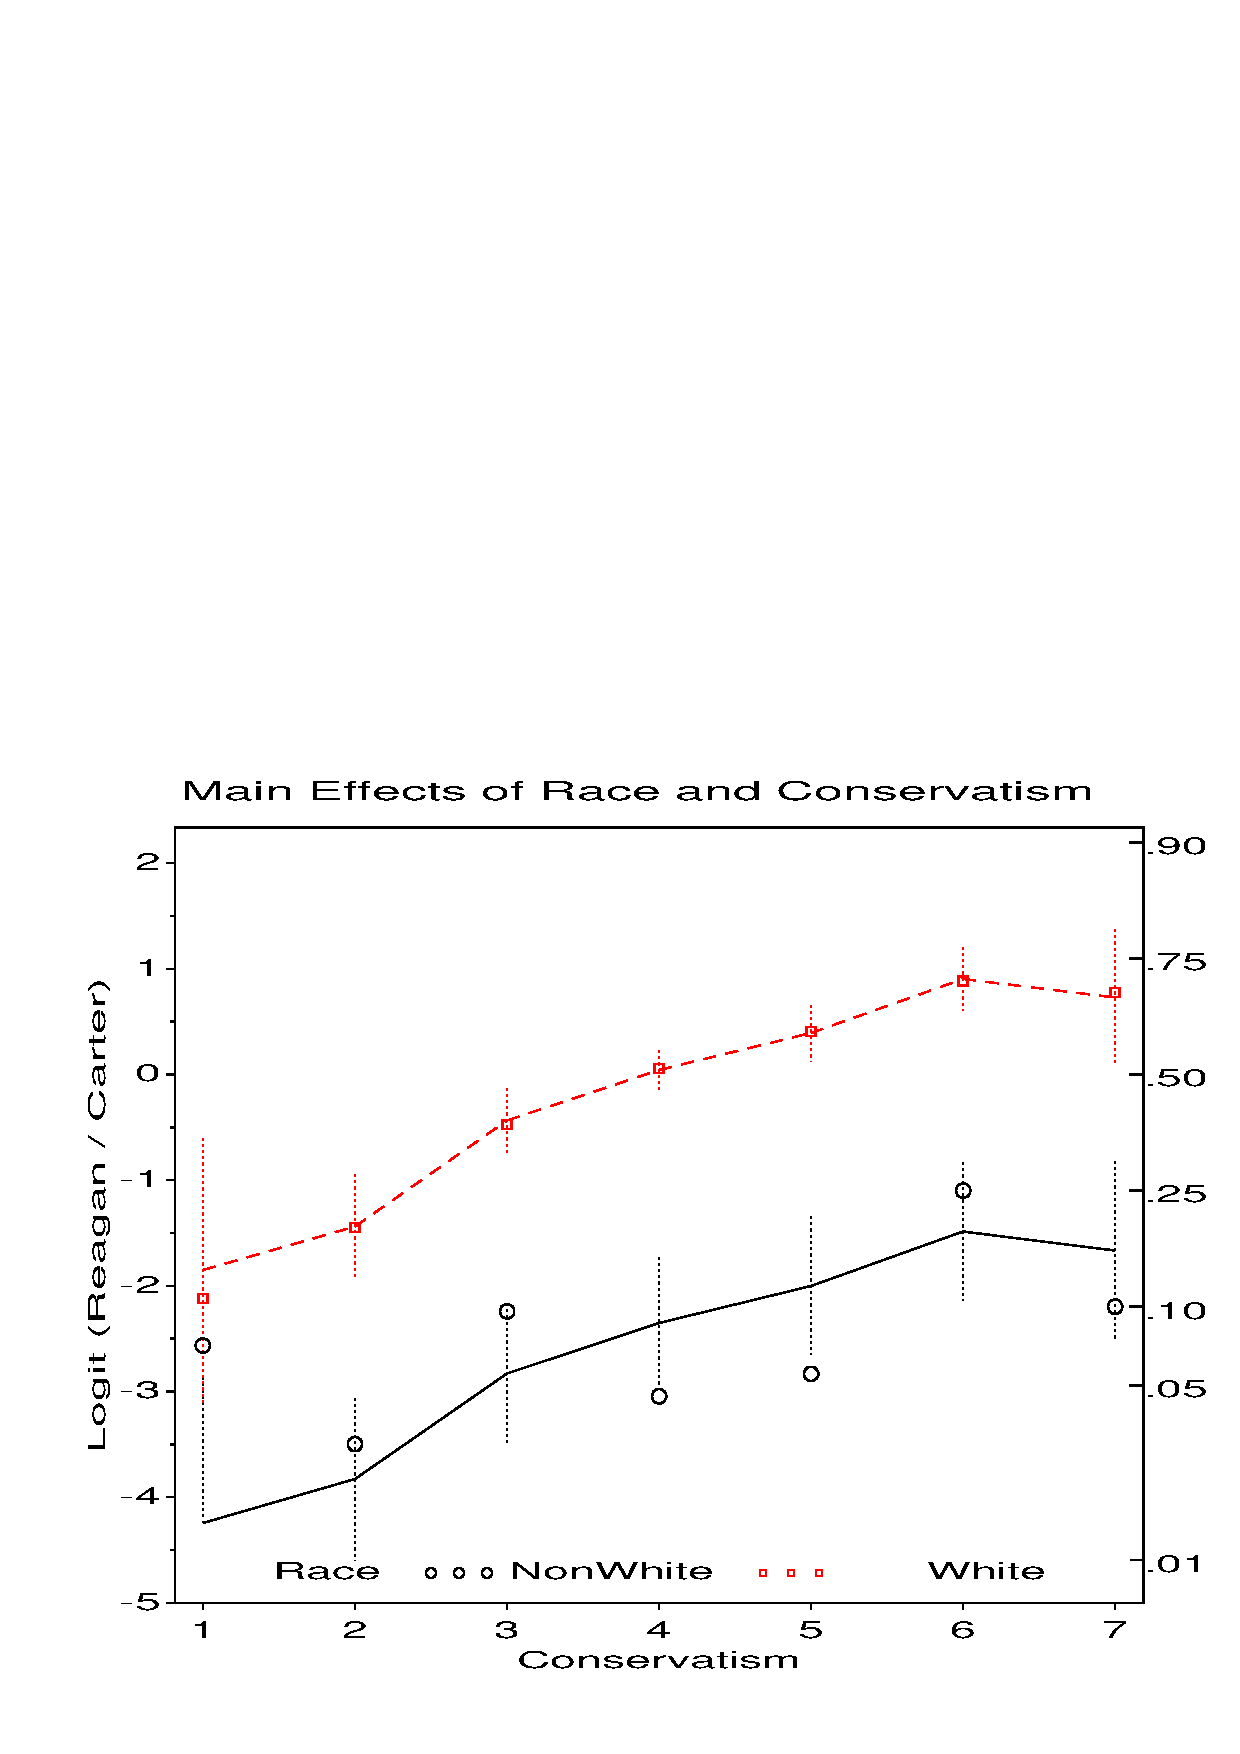
\includegraphics[scale=.6]{glogit11}
  \caption[Observed and fitted logits for main effects model]{Observed (points) and fitted (lines) logits for main effects model.  Dotted lines show a 90\% confidence interval around the predicted log odds.}%
  \label{fig:glogit11}
\end{figure}
Notice that for both Whites and Non Whites, the log odds of voting for
Reagan increases with conservatism.  This is also reflected in the
parameter estimates for \pname{cons} in \outref{out:glogit1.1},
which increase in approximately equal steps.
Model \eqref{eq:logrnom} does not use the ordinal nature of conservatism.
A model which uses conservatism as a direct,
quantitative independent variable ($c$) can be expressed as

\begin{equation} \label{eq:logrlin}
  \mbox{logit ( Reagan / Carter )}  =
  \alpha   +
  \beta _i^{\mbox{\scriptsize Race}}  +
  \beta ^{\mbox{\scriptsize Cons}} \,  c
\end{equation}
Note that there is just one parameter for conservatism,
$ \beta ^{\mbox{\scriptsize Cons}}$, which is interpreted as
an increase in the log odds of a vote for Reagan for each
change of 1 unit in conservatism.
Model \eqref{eq:logrlin} may be fit with \PROC{CATMOD}
just by adding the statement \pname{DIRECT CONS;}
\begin{listing}
proc catmod data=vote order=data;
   direct cons;
   weight count;
   response / out=predict;
   model votefor = race cons / noiter noresponse noprofile ;
   title 'Linear Effect for Conservatism' h=2.5 a=-90 ' ';
\end{listing}
The \LR\ \GSQ\ for this model is $\GSQ (11) = 9.58$, and
the difference in \GSQ\ for Models
\eqref{eq:logrlin} and \eqref{eq:logrnom} is
$\Delta \GSQ (5) = 6.13$,
so the linear model cannot be rejected, given that the nominal
model fits.  The estimate $\widehat{\beta} ^{\mbox{\scriptsize Cons}} = 0.472$
indicates that the odds of voting for Reagan increase by a factor of
$\exp(0.472) = 1.60$ (60\%) for each step of increasing conservatism.

%\begin{Output}[htb]
%\caption{}\label{out:glogit1.2}
%\small
%\verbatiminput{ch7/out/glogit1.2}
%\end{Output}

The observed and fitted logits are plotted exactly as before, using
the same \macro{CATPLOT} call with the new \ODS\ \pname{predict}.
The plot is shown in \figref{fig:glogit12}.
Note that the 90\% confidence limits around predicted values are
noticeably smaller than in \figref{fig:glogit11}.
This is but one advantage of models for ordinal variable,
which we discuss in the following section.
%% one figure
\begin{figure}[htb]
  \centering
  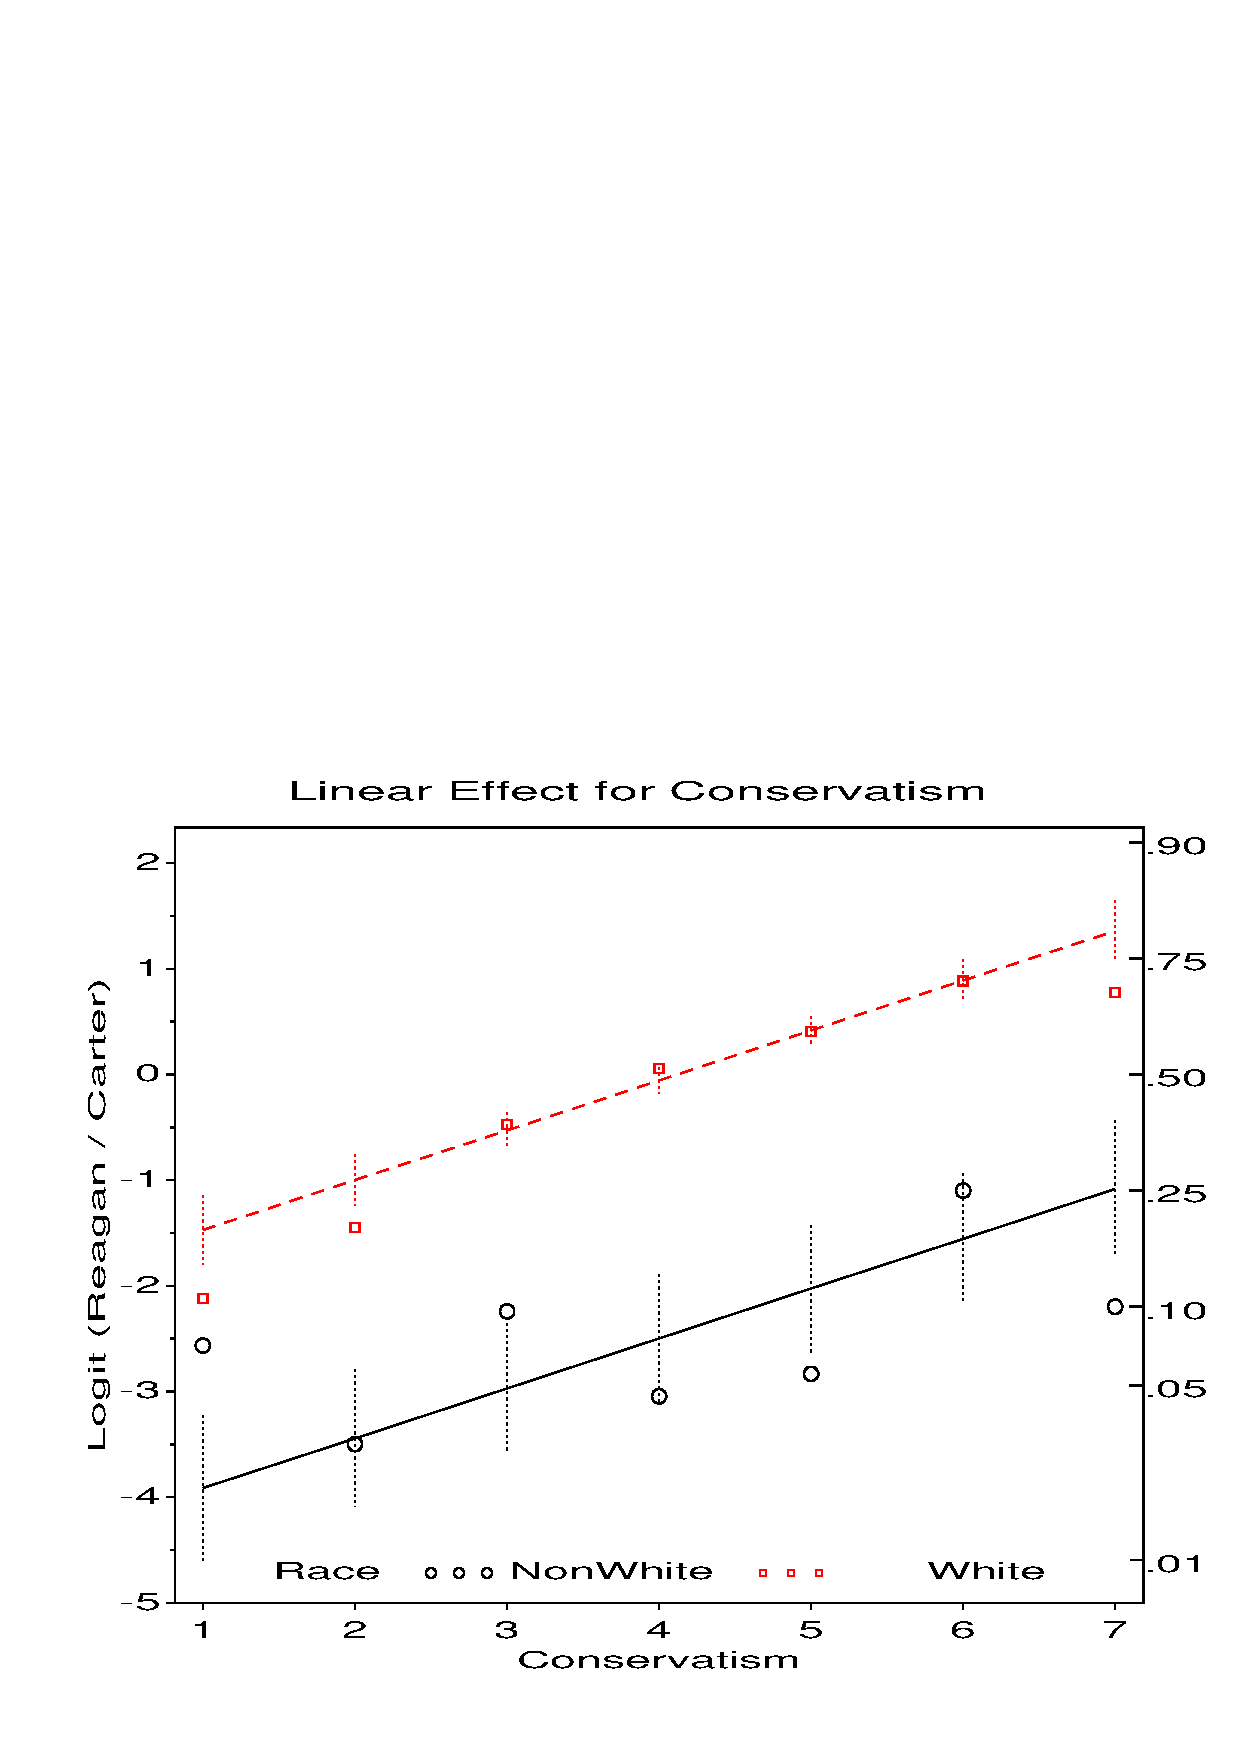
\includegraphics[scale=.6]{glogit12}
  \caption[Observed and fitted logits for linear effect of conservatism]{Observed (points) and fitted (lines) logits for linear effect of conservatism.  Dotted lines show a 90\% confidence interval around the predicted log odds.}%
  \label{fig:glogit12}
\end{figure}
\end{Example}
